\documentclass{article}[18pt]
\usepackage{../../../../../format}
\lhead{A Level Maths - FP2}

\begin{document}
\begin{center}
\underline{\huge Polar Coordinates - Exam Questions}
\end{center}
\section{Example 1 - Finding areas}
\begin{center}
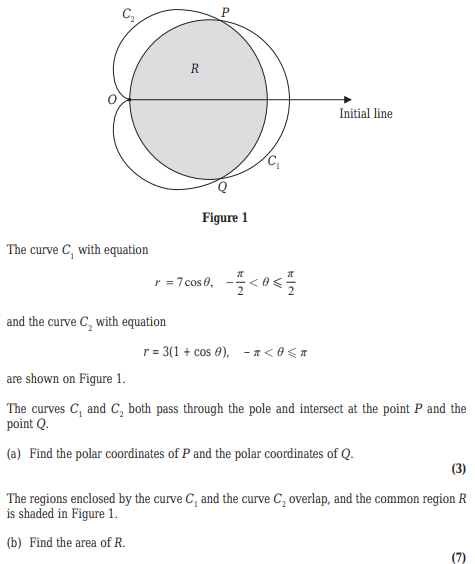
\includegraphics[width=13cm]{Jun16Q8.png}
\end{center}

\textcolor{red}{Set the two curves equal to each other and simplify}
$$7\cos\theta=3(1+\cos\theta)$$
$$4\cos\theta=3$$
$$\cos\theta=\frac{3}{4}$$
\textcolor{red}{Substitute the value of $\cos\theta$ to find the radius}
$$r=7\cos\theta=7\times\frac{3}{4}=\frac{21}{4}$$
\textcolor{red}{Write in polar form}
$$P:\Bigg(\frac{21}{4},0.7727\Bigg) \qquad Q:\Bigg(\frac{21}{4},-0.7227\Bigg)$$
\textcolor{red}{Figure out the areas required to make the area, half the shape and use symmetry to make it easier}
$$C_2:0\leqslant\theta\leqslant\arccos\Bigg(\frac{3}{4}\Bigg)$$
$$C_1:\arccos\Big(\frac{3}{4}\Bigg)\leqslant\theta\leqslant\frac{\pi}{2}$$
\textcolor{red}{Write the integrals required using the formula $A=\frac{1}{2}\int r^2 \ d\theta$}
{\large
$$A=2\Big( \ \frac{1}{2}\int_\alpha^\frac{\pi}{2}(7\cos\theta)^2 \ d\theta+\frac{1}{2}\int_0^\alpha(3(1+\cos\theta))^2 \ d\theta \ \Big)$$}
\textcolor{red}{Multiply through by 2 and expand the brackets}
{\large
$$A=49\int_\alpha^\frac{\pi}{2}\cos^2\theta \ d\theta +9\int_0^\alpha \cos^2\theta+2\cos\theta+1 \ d\theta$$}
\textcolor{red}{Do the integrals}
{\large
$$A=49\Bigg[\frac{1}{2}\sin\theta\cos\theta+\frac{1}{2}\theta\Bigg]^\frac{\pi}{2}_\alpha+9\Bigg[\frac{1}{2}\sin\theta\cos\theta+\frac{3}{2}\theta+2\sin\theta\Bigg]^\alpha_0$$}
\textcolor{red}{Find the values}
$$A=8.62+23.84=32.46$$



\end{document}